\PassOptionsToPackage{colorlinks, unicode, linkcolor=tugreen}{hyperref}
\documentclass[compress, 9pt, aspectratio=1610, professionalfonts]{beamer}

\usepackage{fontspec}
\usepackage{polyglossia}
\setmainlanguage{english}

\usepackage{microtype}

\usepackage{mathtools}
\usepackage[
  math-style=ISO,
  bold-style=ISO,
  nabla=upright,
  partial=upright,
]{unicode-math}
\setmathfont{Tex Gyre Pagella Math}[Scale=MatchLowercase]

\usepackage{csquotes}
\usepackage[
  locale=UK,
  load-configurations=astronomy,
  per-mode=symbol-or-fraction,
]{siunitx}
\DeclareSIUnit{\year}{a}
\AtBeginDocument{%
  \sisetup{%
    math-rm=\mathrm,
  }
}

\usepackage{graphicx}
\usepackage{xcolor}
\colorlet{darkred}{red!80!black}

\usepackage{tikz}
\usetikzlibrary{positioning}
\usetikzlibrary{calc}
\usetikzlibrary{arrows}
\usetikzlibrary{arrows.meta}
\usepackage{pgfplots}

\usepackage[backend=biber, style=verbose]{biblatex}
\addbibresource{references.bib}
\usepackage{hyperref}

\usetheme{tudo}

\newcommand\fullscreenimage[2][]{{%
  \begin{frame}[plain]
    \begin{tikzpicture}[remember picture, overlay, shift=(current page.south west)]
      \fill[black] (0, 0) rectangle (\paperwidth, \paperheight);
      \node[anchor=center] at (current page.center) {%
        \includegraphics[
          width=\paperwidth,
          height=\paperheight,
          keepaspectratio,
        ]{#2}%
      };%
      \node[anchor=south east] at (current page.south east) {#1};%
    \end{tikzpicture}
  \end{frame}%
}}


\tikzset{%
  invisible/.style={opacity=0,text opacity=0},
  visible on/.style={alt={#1{}{invisible}}},
  alt/.code args={<#1>#2#3}{%
    \alt<#1>{\pgfkeysalso{#2}}{\pgfkeysalso{#3}} % \pgfkeysalso doesn't change the path
  },
}

\newcommand\freepicture[3]{%
  \begin{tikzpicture}[remember picture, overlay, shift=(current page.south west)]
    \node[anchor=center] at (#1\paperwidth, #2\paperheight) {#3};
  \end{tikzpicture}%
}

\newcommand\Photon{\ensuremath{\symup{γ}}}
\newcommand\Proton{\ensuremath{\symup{p}}}
\newcommand\Muon{\ensuremath{\symup{μ}}}


\author[M.\ Nöthe]{\textit{Maximilian Nöthe}, Kai Brügge for the FACT-Collaboration}
\date[20.2.2018]{HAP Workshop – Big Data Science in Astroparticle Research – 2018}
\title{FACT Open Data}
\titlegraphic{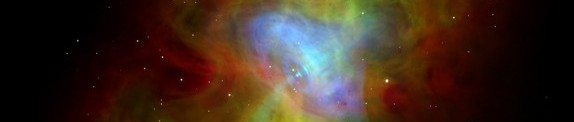
\includegraphics[width=\linewidth]{images/crab_title.jpg}}

\institute[%
  {
\includegraphics[height=\headerheight]{logos/fact.pdf}}%
  \hspace{1em}%
  {
\includegraphics[height=\headerheight]{logos/sfb876.pdf}}%
  \hspace{1em}%
  {
\includegraphics[height=\headerheight]{logos/e5logo.pdf}}%
]{
  {\includegraphics[height=0.75cm]{tu.pdf}}%
  \hspace{1em}%
  {
\includegraphics[height=0.75cm]{logos/ethz.pdf}}%
  \hspace{1em}%
  {
\includegraphics[height=0.75cm]{logos/isdc.pdf}}%
  \hspace{1em}%
  {
\includegraphics[height=0.75cm]{logos/uniwue.pdf}}%
}

\begin{document}
\begin{frame}
  \maketitle
\end{frame}

\begin{frame}{Overview}
  \begin{columns}[c, onlytextwidth]
    \begin{column}{0.66\textwidth}
      \linespread{1.5}
      \tableofcontents[hideallsubsections]
    \end{column}
    \hfill
    \begin{column}{0.33\textwidth}
      \raggedleft
      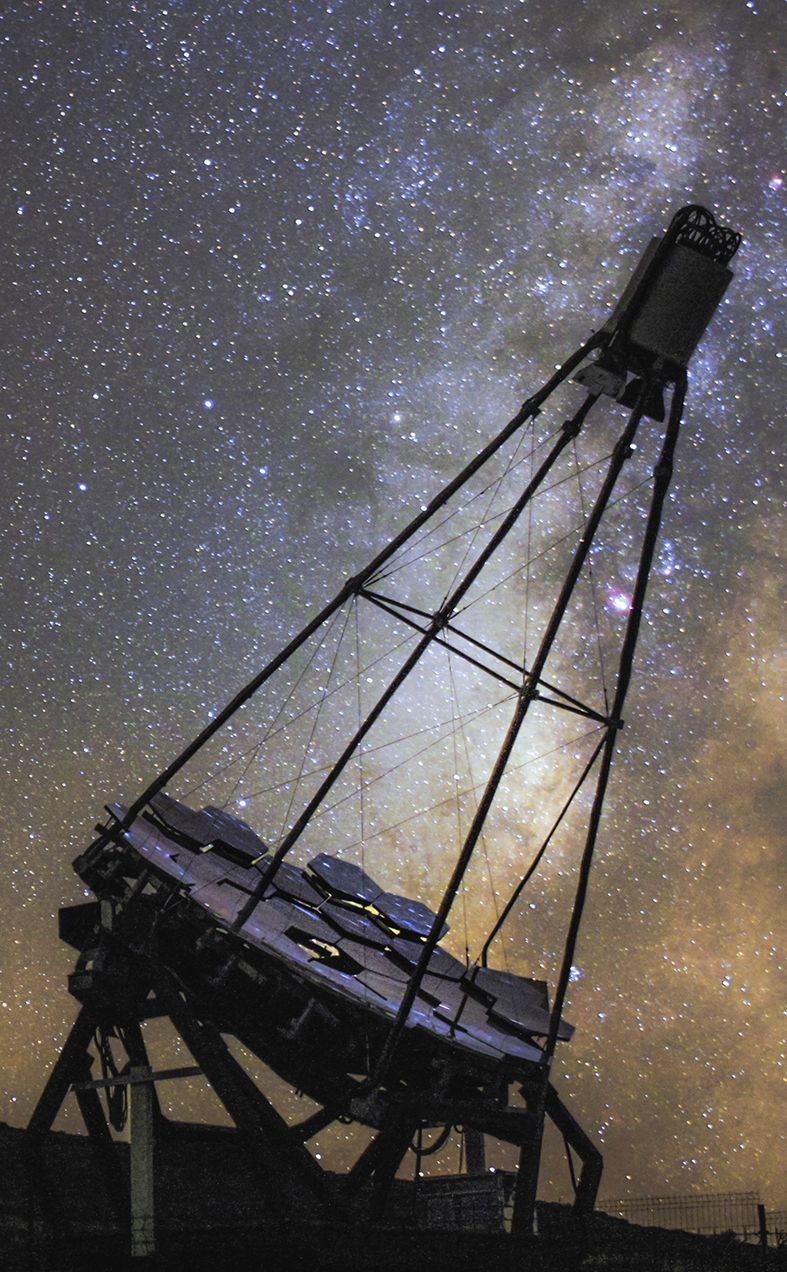
\includegraphics[height=0.85\textheight]{fact_claro_crop.jpg}\\
      {\tiny[Miguel Claro]}
    \end{column}
  \end{columns}
\end{frame}

\section{Introduction}
\begin{frame}
  \begin{center}
    \begin{tikzpicture}
      \large
\coordinate (mirror) at (4.1, 3.95);
\coordinate (cameracenter) at (8.4, 4.6);

\node[anchor=south west,inner sep=0] (background) at (0, 0) {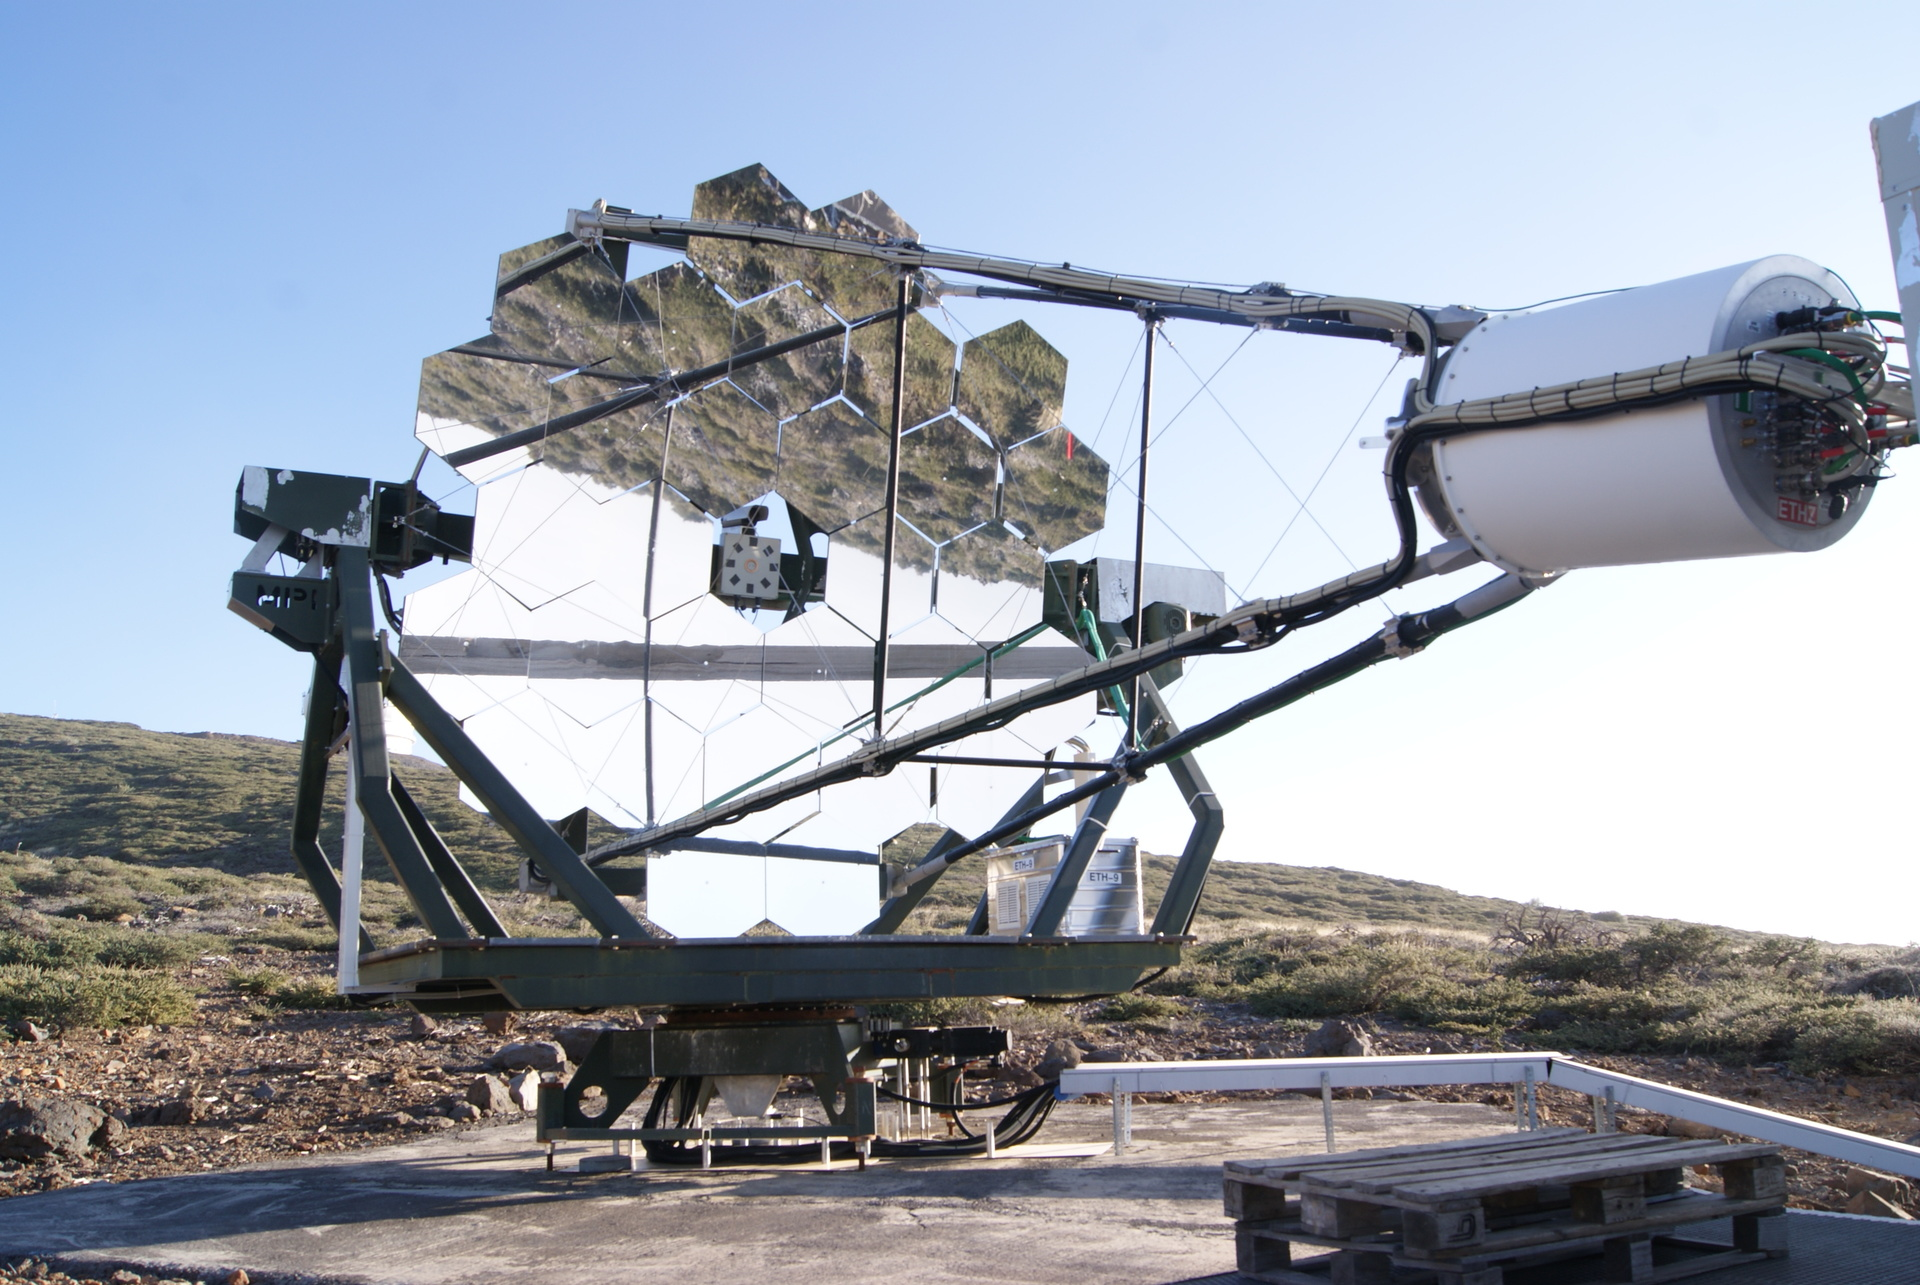
\includegraphics[height=0.92\textheight]{images/fact.jpg}};


\node[anchor=south west,inner sep=0] (camera) at (7, 0.5) {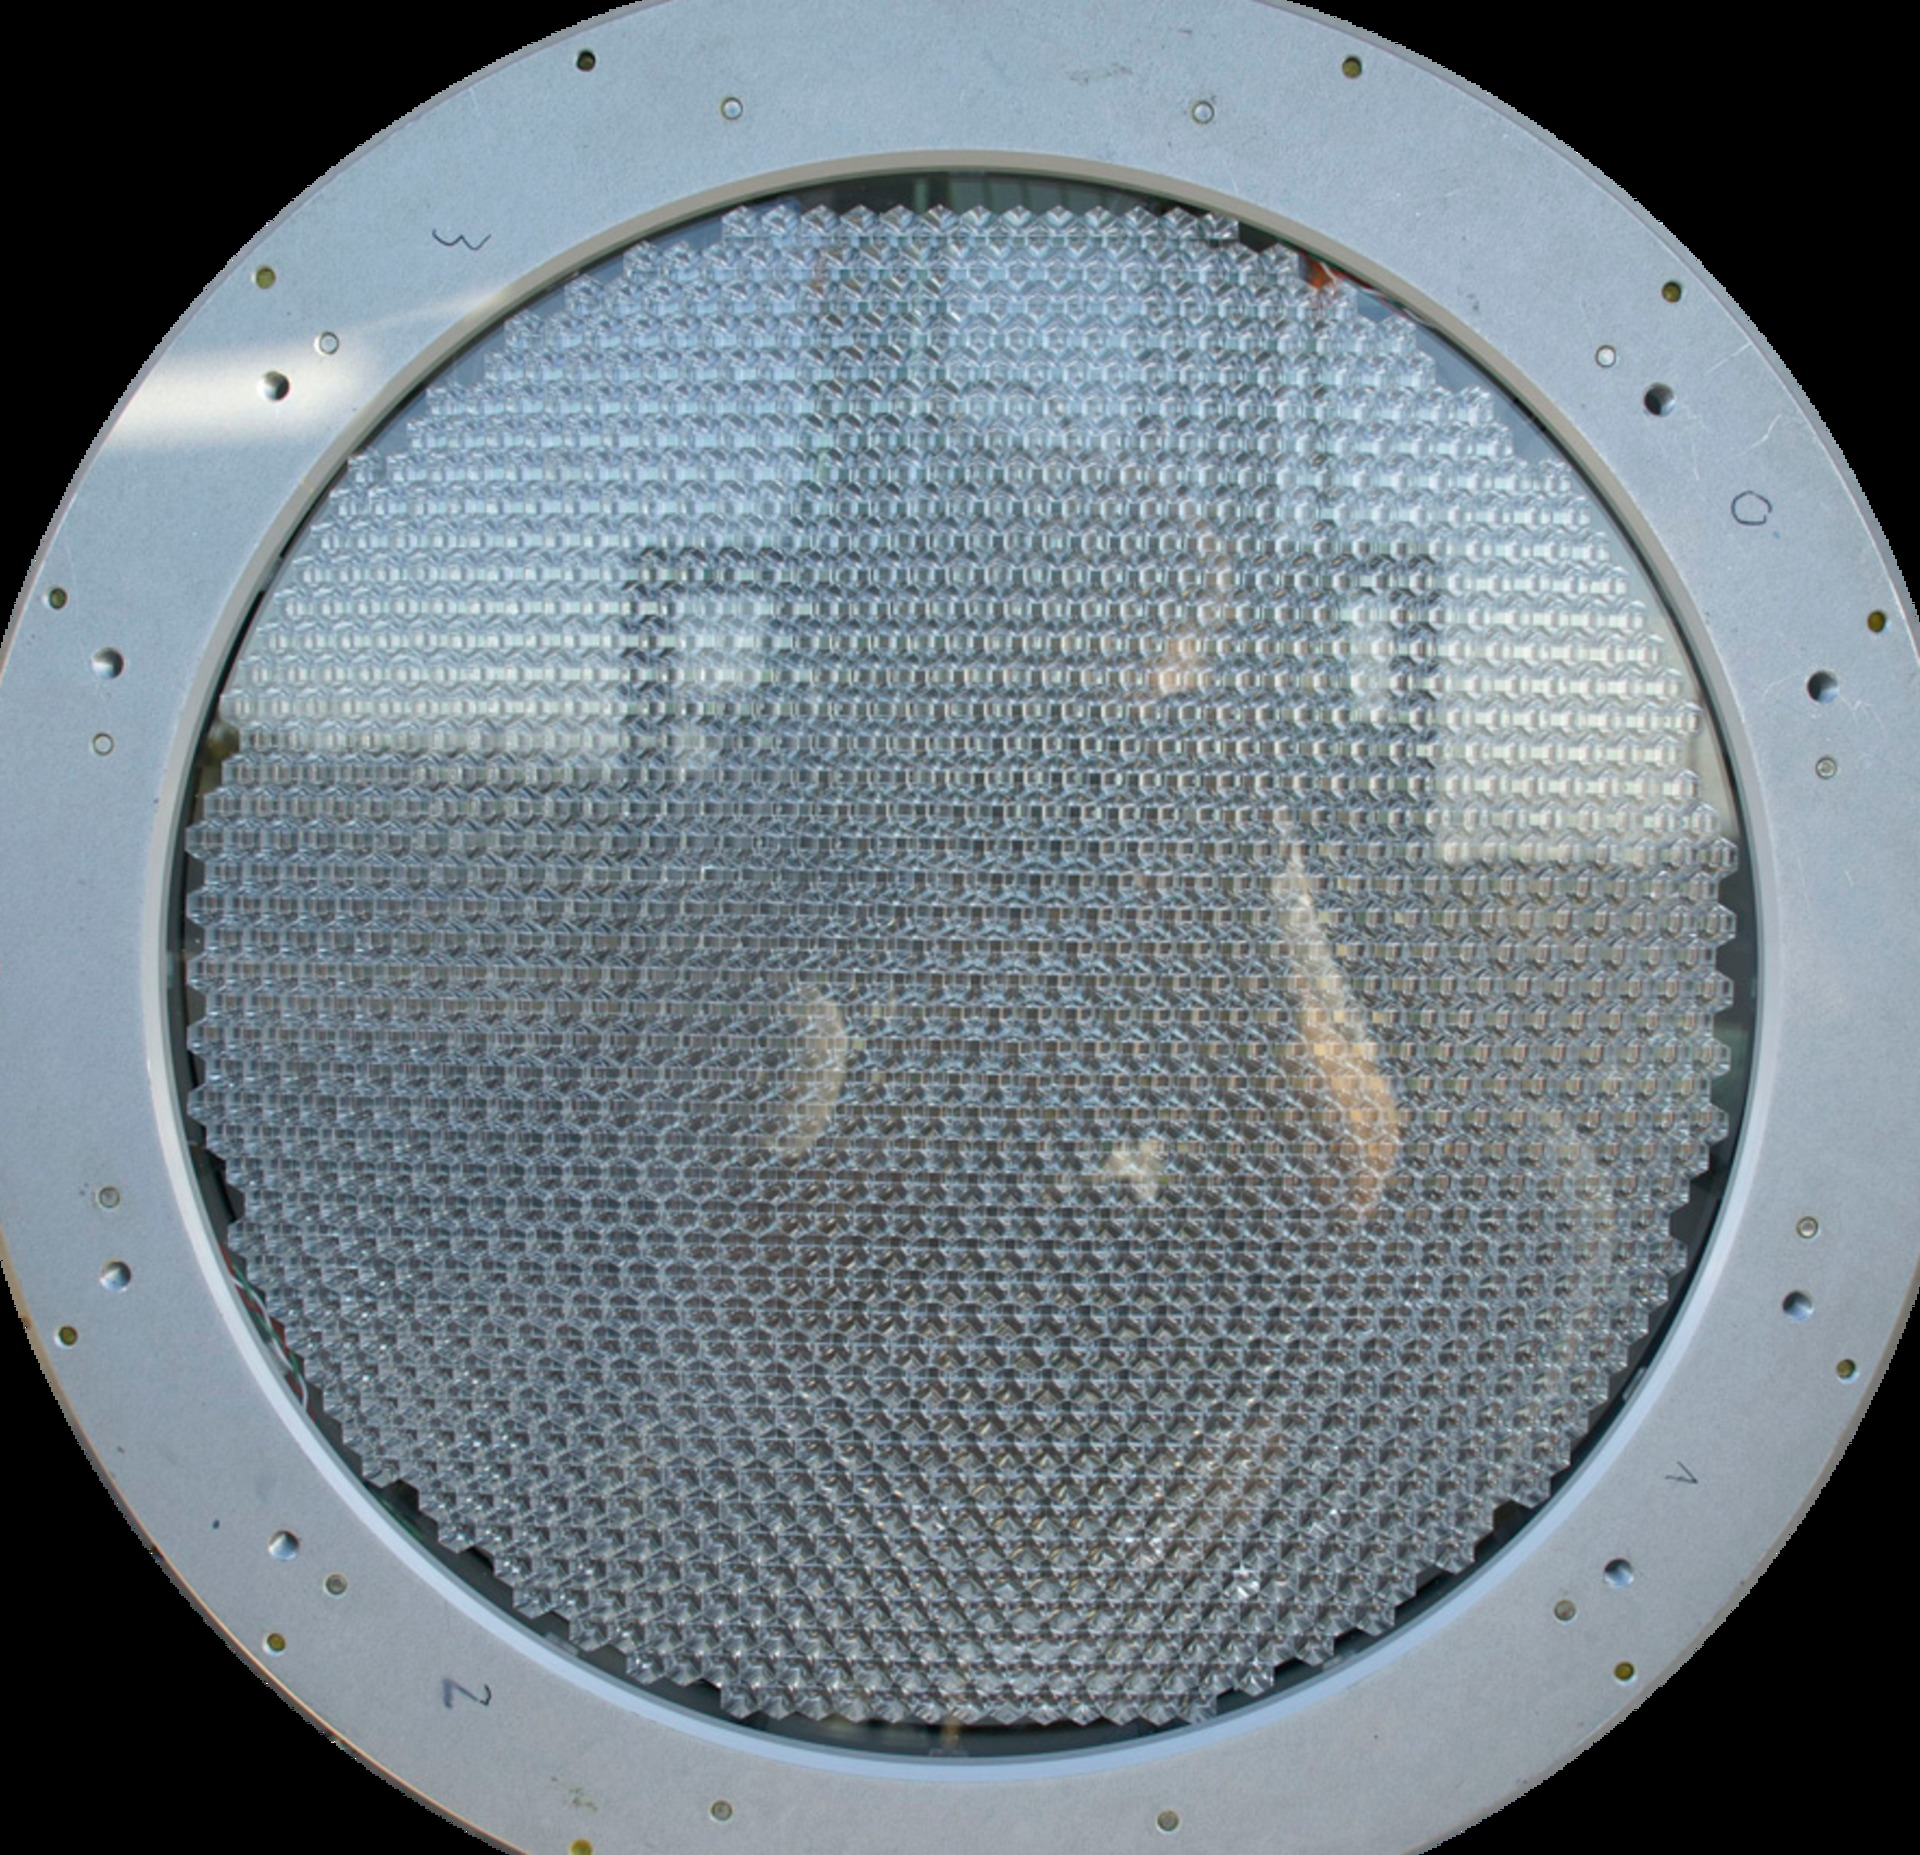
\includegraphics[width=0.2\textwidth]{images/camera.jpg}};



\draw[very thick,tugreen] (mirror) circle (2.05);
%\draw[thick,tugreen] (4,3.75) circle (0.05);
\draw[very thick,tugreen, rotate around={45:(mirror)}] ($(mirror)-(2.05,0)$) --
  ($(mirror)+(2.05,0)$)
  node[midway, above, black, fill=white, fill opacity=0.7, text opacity=1, rotate=45, rounded corners,]{$\diameter = \SI{3.8}{\meter}$};



\draw[very thick,tugreen] (cameracenter) ellipse (0.58 and 0.73);
%\draw[thick,tugreen] (7.9,4.4) circle (0.05);
\draw[very thick,tugreen] ($(cameracenter)-(0.58,0)$) to ($(camera.west)-(0.005*\textwidth,0)$);
\draw[very thick,tugreen] ($(cameracenter)+(0.58,0)$) to ($(camera.east)+(0.005*\textwidth,0)$);
\draw[very thick,tugreen] (camera.center) circle (0.105\textwidth);

\node[black,anchor=south west, fill=white, rounded corners] at (0.6,0.15) {\textbf{Roque des los Muchachos, La Palma}};


\node[black,anchor=center,text centered, fill=white, fill opacity=0.7, text opacity=1, rounded corners] at (camera.center) {\textbf{1440 Pixel}};
\node[black,anchor=east,text centered] at (9.9,6.4) {\textbf{1 Pixel = 1 SiPM = 3600 G-APDs}};

    \end{tikzpicture}
  \end{center}
\end{frame}

\section{Dataset Overview}
\begin{frame}[c]{The Dataset}
  \begin{columns}[onlytextwidth]
    \begin{column}{0.55\textwidth}      
      \begin{itemize}
        \item Crab Observations from November 2013
        \item Point-source gamma-ray simulations
        \item Diffuse gamma-ray simulations
        \item Diffuse proton simulations
        \item Available in different formats and multiple analysis stages
      \end{itemize}
    \end{column}
    \hfill
    \begin{column}{0.4\textwidth}      
      \hfill
      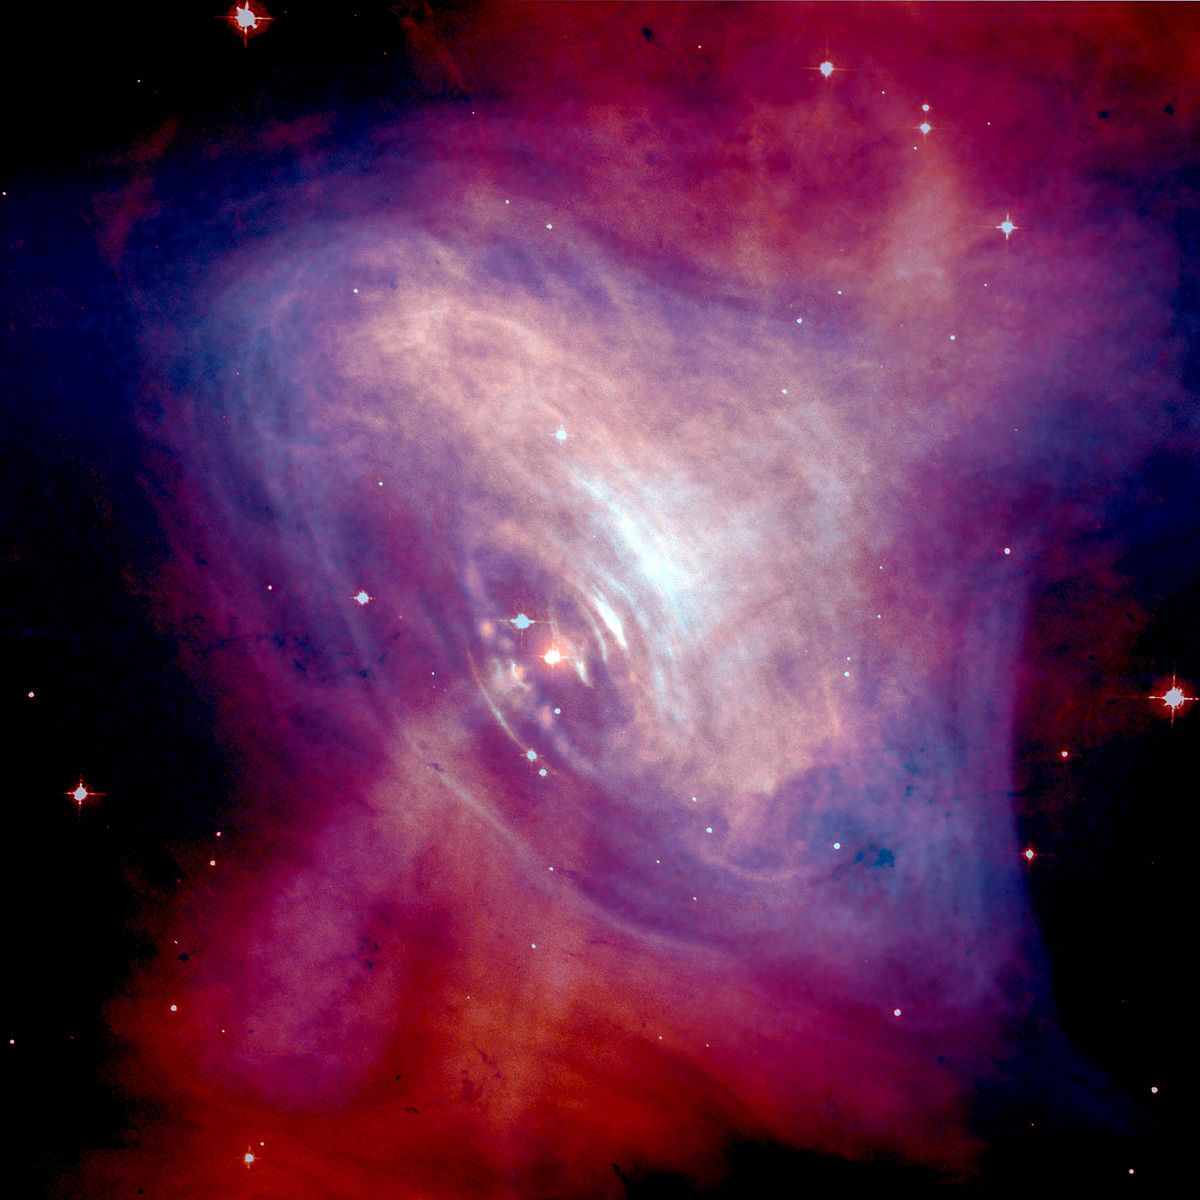
\includegraphics[width=0.75\textheight]{images/crab_chandra.jpg}
    \end{column}
  \end{columns}
  \vspace{0.5cm}
  \begin{center}
    \LARGE\url{https://fact-project.org/data}
  \end{center}
\end{frame}

\begin{frame}[c]{Observations}
  \begin{columns}[onlytextwidth]
    \begin{column}{0.475\textwidth}      
      \begin{itemize}
        \item \num{17.7} hours of Crab Nebula observations
        \item Good environmental conditions
        \item Zenith distance between \ang{6} and \ang{30}
      \end{itemize}
      \vspace{0.25cm}
      \begin{center}
        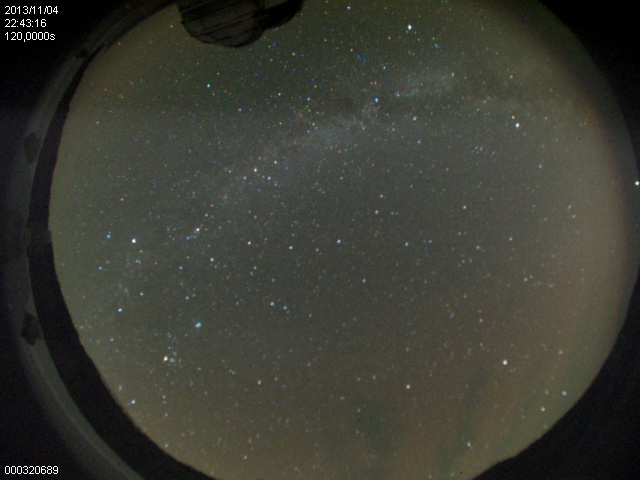
\includegraphics[width=0.75\linewidth]{images/gtc.jpg}
      \end{center}
    \end{column}
    \hfill
    \begin{column}{0.475\textwidth}      
      \includegraphics{build/plots/zenith.pdf}
    \end{column}
  \end{columns}
  
\end{frame}

\begin{frame}[t]{Simulations}
  \begin{itemize}
    \item CORSIKA for air shower simulations
    \item CERES for FACT detector response simulations
  \end{itemize}

  \vspace{1cm}

  \begin{columns}[onlytextwidth]
    \begin{column}{0.475\textwidth}
      \textcolor{tugreen}{\Large Gammas}
      \begin{description}[Triggered Events]
        \item[Energy Range] \SI{200}{\GeV} – \SI{50}{\TeV}
        \item[Spectral Slope] \num{-2.7}
        \item[Max. Impact] \SI{270}{\meter}
        \item[Zenith Distance] \ang{0} – \ang{30}
        \item[CORSIKA Events] \num{12000000}
        \item[Triggered Events] \num{1914812}
      \end{description}
    \end{column}
    \hfill
    \begin{column}{0.475\textwidth}
      \textcolor{tugreen}{\Large Protons}
      \begin{description}[Triggered Events]
        \item[Energy Range] \SI{100}{\GeV} – \SI{200}{\TeV}
        \item[Spectral Slope] \num{-2.7}
        \item[Max. Impact] \SI{400}{\meter}
        \item[Zenith Distance] \ang{0} – \ang{30}
        \item[CORSIKA Events] \num{780046520}
        \item[Triggered Events] \num{509652}
      \end{description}
    \end{column}
  \end{columns}
\end{frame}

\begin{frame}[t]{A FACT Analysis}
  \begin{columns}[onlytextwidth]
    \begin{column}{0.475\textwidth}
      Classical IACT Analysis Chain
      \begin{enumerate}
        \item Raw Data Calibration
        \item Removal of electronic artifacts
        \item Extraction of number of photons and mean arrival times for each pixel
        \item Image parameterization
        \item Reconstruction of particle properties
          \begin{itemize}
            \item Energy
            \item Origin
            \item Particle type (\Photon, \Proton, \Muon)
          \end{itemize}
      \end{enumerate}
    \end{column}
    \hfill
    \begin{column}{0.475\textwidth}%
      \only<1>{\includegraphics{build/plots/drs_calib.pdf}}%
      \only<2>{\includegraphics{build/plots/spikes.pdf}}%
      \only<3>{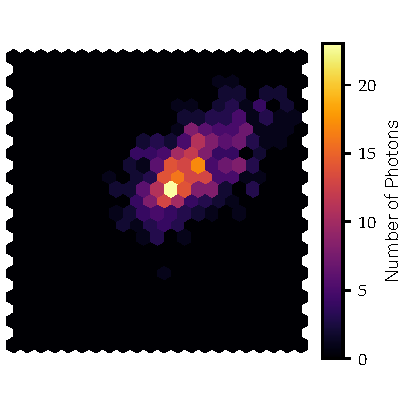
\includegraphics{images/hillas_1.pdf}}%
      \only<4>{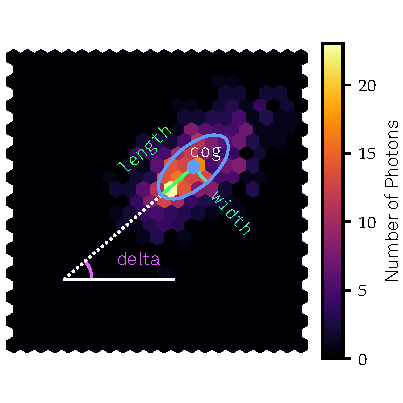
\includegraphics{images/hillas_2.pdf}}%
    \end{column}%
  \end{columns}
\end{frame}

\section{Data Formats}
\begin{frame}[t]{Raw Data}
  \begin{itemize}
    \item FACT observations are stored in custom compressed FITS Files called \texttt{zfits}\\
    \item Readers are available for
      \begin{description}
        \item[Python] \url{https://github.com/fact-project/zfits} 
        \item[Java] \url{https://github.com/fact-project/fact-tools} 
        \item[C++ (ROOT)] \url{https://trac.fact-project.org/browser/trunk/Mars} 
      \end{description}
    \item FACT-Tools can be easily used to convert \texttt{zfits} to standard FITS
    \item Simulations are stored in standard, gzipped FITS Files
    \item Raw Data consists of a single array of length $1440 \times 300$ ($N_\text{Pixels} \times N_\text{Slices}$)

      \begin{center}
        \begin{tikzpicture}
          \foreach \i in {0,...,2} {
            \node[anchor=west, minimum width=0.5cm, minimum height=0.5cm, fill=blue!20, draw=black] at (\i * 0.5cm, 0) {\tiny \i};
          }
          \node[anchor=west, minimum width=0.5cm, minimum height=0.5cm] at (1.5cm, 0) {$\cdots$};
          \foreach \j in {298,299} {
            \node[anchor=west, minimum width=0.5cm, minimum height=0.5cm, fill=blue!20, draw=black] at (\j * 0.5cm - 147cm, 0) {\tiny \j};
          }
          \foreach \i in {0,...,2} {
            \node[anchor=west, minimum width=0.5cm, minimum height=0.5cm, fill=green!20, draw=black] at (\i * 0.5cm + 3cm, 0) {\tiny \i};
          }
          \node[anchor=west, minimum width=0.5cm, minimum height=0.5cm] at (4.5cm, 0) {$\cdots$};
          \foreach \j in {298,299} {
            \node[anchor=west, minimum width=0.5cm, minimum height=0.5cm, fill=green!20, draw=black] at (\j * 0.5cm - 144cm, 0) {\tiny \j};
          }
          \node[anchor=west, minimum width=0.5cm, minimum height=0.5cm] at (6cm, 0) {$\cdots$};
          \node at (1.5cm, -0.5cm) {Pixel 0};
          \node at (4.5cm, -0.5cm) {Pixel 1};
        \end{tikzpicture}
      \end{center}
  \end{itemize}
    
  \begin{center}
    \small See: \cite{zfits}
  \end{center}
\end{frame}

\begin{frame}[c]{Photon Stream}
  \begin{columns}[onlytextwidth]
    \begin{column}{0.475\textwidth}
      \begin{itemize}
        \item The FACT Camera has single photon resolution
        \item Each photon produces a known pulse shape 
        \item Multiple photons just superimpose
        \item[→] Reconstruct the arrival time of each individual photon by subtracting pulses until a flat line is reached
      \end{itemize}
      \begin{center}
        \small See: \cite{photonstream}
      \end{center}
    \end{column}
    \begin{column}{0.475\textwidth}
      \includegraphics{build/plots/phs.pdf}
    \end{column}
  \end{columns}
\end{frame}

\section{FACT-Tools Standard Analysis}
\begin{frame}[t]{FACT-Tools}
\end{frame}

\begin{frame}[t]{Higher-Level Analysis}
\end{frame}

\section{Outlook \& Conclusion}

\begin{frame}[t]{Deep Learning}
\end{frame}

\end{document}
